% Gemini theme
% https://github.com/anishathalye/gemini

\documentclass[final]{beamer}

% ====================
% Packages
% ====================

\usepackage[T1]{fontenc}
\usepackage{lmodern}
\usepackage[size=custom,width=120,height=72,scale=1.0]{beamerposter}
\usetheme{gemini}
\usecolortheme{gemini}
\usepackage{graphicx}
\usepackage{booktabs}
\usepackage{tikz}
\usepackage{pgfplots}

\DeclareMathOperator*{\argmax}{\arg\max}

% ====================
% Lengths
% ====================

% If you have N columns, choose \sepwidth and \colwidth such that
% (N+1)*\sepwidth + N*\colwidth = \paperwidth
\newlength{\sepwidth}
\newlength{\colwidth}
\setlength{\sepwidth}{0.025\paperwidth}
\setlength{\colwidth}{0.3\paperwidth}

\newcommand{\separatorcolumn}{\begin{column}{\sepwidth}\end{column}}

% ====================
% Title
% ====================

\title{BCFW and Dual extragradient, two complementary approaches to structured optimization}
\author{William St-Arnaud\inst{1} \and Fr\'ed\'eric Boileau \inst{1} \and Elyes Lamouchi\inst{1}}

\institute[shortinst]{\inst{1} Universit\'e de Montr\'eal}

% ====================
% Body
% ====================

\begin{document}

\begin{frame}[t]
\begin{columns}[t]
\separatorcolumn

\begin{column}{\colwidth}

  \begin{block}{}

    \begin{figure}
      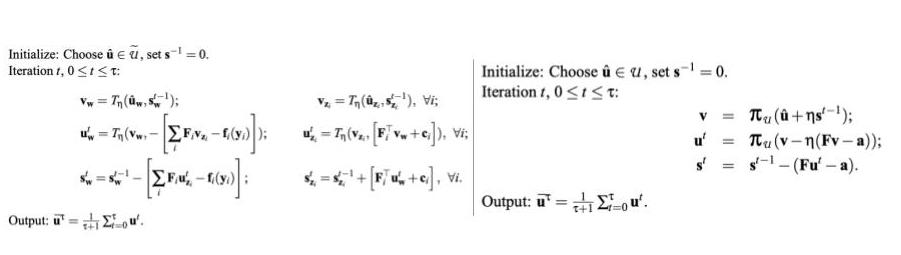
\includegraphics{img/extra_grad.jpg}
      \caption{Dual extragradient algorithm with Euclidean projections and Bregman projections}
      \label{extragrad}
    \end{figure}
  \end{block}


  \begin{block}{Dual extragradiant alogrithm}
    The dual extragradiant takes advantage of the min-max formulation of the
problem. Instead of dualizing the max oracle and peforming FW or projected
gradient descent, we could try alternating between updates for the max and min
(can see them as opponents). However this can lead to oscillation. A better way
would be to combine the two vectors we update alternatively into one and then
perform two gradient udpates. The first one is called a ``look-ahead'' step.
This step consists in starting from a point inside the constraint set and moving
away from it by a little amount and then projecting back to the constraint set.
The second step consists in performing the gradient udpate using the look-ahed
point. Then, we update the trajectory completed so far so that the next
iteration can perform a look-ahead step using that starting point.
    \begin{itemize}
      \item The dual extragradient algorithm takes advantage of the min-max
(saddle-point) formulation. No need to find the dual of one of the objectives.
      \item We can use this formulation on many more problems for which we do not have a parameter space defined
	by linear and convex quadratic constraints which are necessary for using commercial solvers.
    \end{itemize}

    The most intuitive type of projection that can be used is the Euclidean
projection. However, for some problems these are expensive to compute (e.g.
think cuts or matching problems) The method that we present introduces the
concept of Bregman projections. The Bregman projection comes from the Bregman
divergence. The Bregman divergene between $u$ and $u'$ for a strongly convex
function $h$ is simply an upper bound to the squared norm of $u' - u$ :
    \begin{equation*}
      d(u', u) = h(u') - h(u) - \nabla h(u)^T (u' - u) \geq \lVert u' - u \rVert^2
    \end{equation*}
    The Bregman projection is then the following operator:
    \begin{equation*}
      T_{\eta}(u,s) = \argmax_{u' \in \mathcal{U}} \left[ s^T (u' - u) - \frac{1}{\eta} d(u', u)\right]
      \end{equation*}
    \begin{itemize}
      \item Bregman projections are easier to derive a projection for some
problems where Euclidean projections are hard (e.g. matchings)
      \item We only need a strongly convex function for the norm on the combined
parameters (i.e. $u = (w,z)$).
    \end{itemize}
  \end{block}
\end{column}

\separatorcolumn

\begin{column}{\colwidth}

  \begin{alertblock}{Face Expression Comparison dataset (FEC)}
    In our experiments, we used the FEC dataset. It consists of 3-tuples of face
images. In each tuple, a person has labeled the the two images that likely
depict the same emotion. The emotion labels of each image were picked from
another dataset. The 3-tuples are labeled as ONE-CLASS, TWO-CLASS, or
THREE-CLASS. This simply tells us how many emotions are shown in the three
images. The data was split into a training set and a test set.

    We extracted all images and resized them to $32 \times 32$ images to have a
fixed dimension for the features. The feature vectors were then simply a
concatenation of two flattened images. As there were three labels possible (e.g.
1-2, 1-3, and 2-3), we had three possible features per 3-tuple. The size of the
feature vectors was thus $32
\times 32 \times 2 = 2048$

    \begin{figure}
      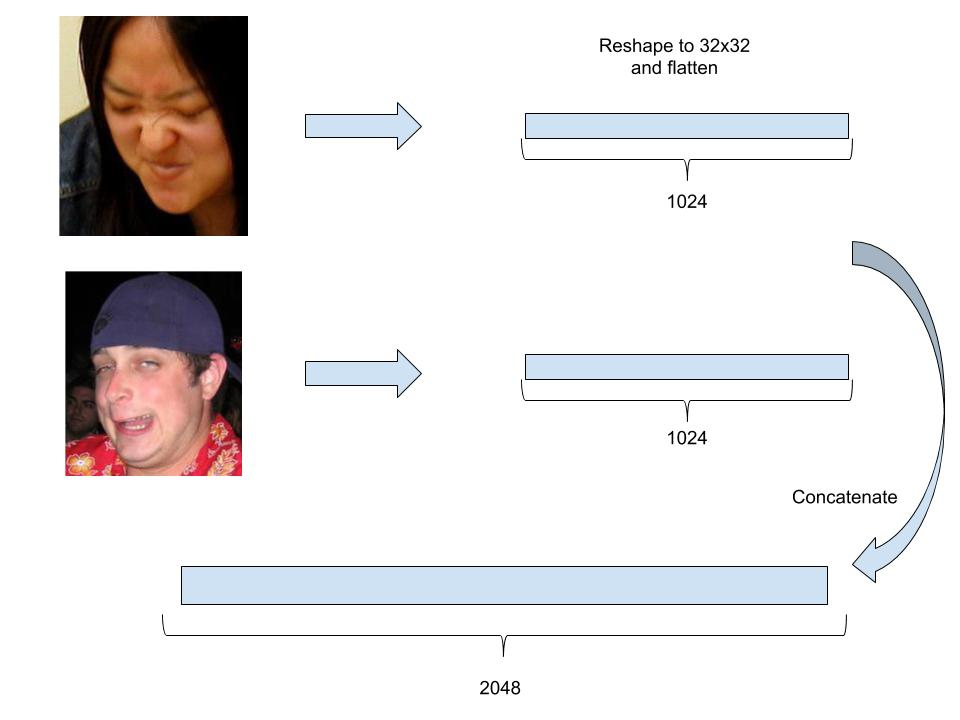
\includegraphics[scale=0.75]{img/fec_poster.jpg}
      \caption{How the feature vectors are extracted from two images}
      \label{feat_vec}
    \end{figure}
  \end{alertblock}

\end{column}

\separatorcolumn

\begin{column}{\colwidth}

  \begin{block}{Block-coordinate Frank-Wolfe}
    The BCFW algorithm takes advantage of the shape of the constraints of the
optimization problem. If they can separated in independent blocks, we can view
smaller optimization problems for each block and recombine later to find a
solution to the main problem.

    $$
    \int_{-\infty}^{\infty} e^{-x^2}\,dx = \sqrt{\pi}
    $$

    Interdum et malesuada fames $\{1, 4, 9, \ldots\}$ ac ante ipsum primis in
    faucibus. Cras eleifend dolor eu nulla suscipit suscipit. Sed lobortis non
    felis id vulputate.

    \heading{A heading inside a block}

    Praesent consectetur mi $x^2 + y^2$ metus, nec vestibulum justo viverra
    nec. Proin eget nulla pretium, egestas magna aliquam, mollis neque. Vivamus
    dictum $\mathbf{u}^\intercal\mathbf{v}$ sagittis odio, vel porta erat
    congue sed. Maecenas ut dolor quis arcu auctor porttitor.

    \heading{Another heading inside a block}

    Sed augue erat, scelerisque a purus ultricies, placerat porttitor neque.
    Donec $P(y \mid x)$ fermentum consectetur $\nabla_x P(y \mid x)$ sapien
    sagittis egestas. Duis eget leo euismod nunc viverra imperdiet nec id
    justo.

  \end{block}

  \begin{block}{Nullam vel erat at velit convallis laoreet}

    Class aptent taciti sociosqu ad litora torquent per conubia nostra, per
    inceptos himenaeos. Phasellus libero enim, gravida sed erat sit amet,
    scelerisque congue diam. Fusce dapibus dui ut augue pulvinar iaculis.

    \begin{table}
      \centering
      \begin{tabular}{l r r c}
        \toprule
        \textbf{First column} & \textbf{Second column} & \textbf{Third column} & \textbf{Fourth} \\
        \midrule
        Foo & 13.37 & 384,394 & $\alpha$ \\
        Bar & 2.17 & 1,392 & $\beta$ \\
        Baz & 3.14 & 83,742 & $\delta$ \\
        Qux & 7.59 & 974 & $\gamma$ \\
        \bottomrule
      \end{tabular}
      \caption{A table caption.}
    \end{table}

    Donec quis posuere ligula. Nunc feugiat elit a mi malesuada consequat. Sed
    imperdiet augue ac nibh aliquet tristique. Aenean eu tortor vulputate,
    eleifend lorem in, dictum urna. Proin auctor ante in augue tincidunt
    tempor. Proin pellentesque vulputate odio, ac gravida nulla posuere
    efficitur. Aenean at velit vel dolor blandit molestie. Mauris laoreet
    commodo quam, non luctus nibh ullamcorper in. Class aptent taciti sociosqu
    ad litora torquent per conubia nostra, per inceptos himenaeos.

    Nulla varius finibus volutpat. Mauris molestie lorem tincidunt, iaculis
    libero at, gravida ante. Phasellus at felis eu neque suscipit suscipit.
    Integer ullamcorper, dui nec pretium ornare, urna dolor consequat libero,
    in feugiat elit lorem euismod lacus. Pellentesque sit amet dolor mollis,
    auctor urna non, tempus sem.

  \end{block}

  \begin{block}{References}

    \nocite{*}
    \footnotesize{\bibliographystyle{plain}\bibliography{poster}}

  \end{block}

\end{column}

\separatorcolumn
\end{columns}
\end{frame}

\end{document}
